\chapter{Simulating interaction between CSF and the Spinal Cord}
\section{Overview of previous studies}
To our knowledge, few studies has investigated fluid-structure interaction modeling of the CSF and the spinal cord including a syrinx. 
\\
\\
Some studies have investigated the effects of FSI on the spinal cord movement and CSF pressure in geometries without a syrinx. Clark \cite{Clar13} assumed the Youngs modulus to be 1 MPa for the spinal cord, and in their initial tests this choice caused only small displacements. Therefore the conclusion was that FSI had a negligible effect on CSF pressure in the SAS. \\
Cheng et al. \cite{Chen14} investigated FSI effects on a patient-specific 3D-geometry. In their model they assumed a Youngs modulus of 0.7 MPa, and reached the same conclusion as Clark. As highlighted: \textit{"This study informs that fluid structure interaction has no effect on CSF pressure"}. 
\\ Clearly, a too high elastic modulus will undermine the effects of FSI, if they do exist. Considering the wide range of material parameters reported in the literature for the spinal cord, we believe further investigation is necessary to be able to make such a statement. In addition, these two studies does not seem to investigate syringomelia as a primary target, and therefore important effects of FSI could have been overlooked in these specific cases. It has correctly been argued that the pressures involved in these studies ($<100 Pa$) are almost negligible in magnitude compared to even the lowest estimates of the elastic modulus of the Spinal cord ($>5kPa$). This should cause only very small discplacements, and this also seem to be the case for healthy subjects. However, when the syrinx is large, there is only a thin membrane of spinal cord tissue separating the SAS and the fluid in the syrinx allowing larger cord movements.  \\
\\
\\
In porous models presented by Dr{\o}sdal, \cite{Dros11} fluid pressure within the cord was altered by the presence of a syrinx but the CSF pressure in the SAS was not. velocities up to only 3e-7 cm/s inside the syrinx was reported, and therefore there must be some other effects causing the more rapid fluid movement inside the syrinx.  
\\
\\
To our knowledge, the most noted group working on FSI effects on Syringomelia include the group of Chris D. Bertram at the University of Sydney. Some of their work include research on pressure waves propagating in the spinal cord in the presence of a syrinx \cite{Bert05},\cite{Bert08},\cite{Bert09}. Even though, in this series of papers the main focus is on the overlap between the cervical and thoracic segments of the spinal cord, the mechanisms of interest remians the same.
\\
\\
Even with today's high quality magnetic resonance imaging, (MRI) or phase contrast MR (PC-MR), exact velocities are hard to measure. Healthy subjects also has very complex CSF flow and thus difficult to observe or quantify. Since the Chiari I malformation is associated with abnormal CSF flow, a realistic model simulating the pre-operative case needs abnormal inflow or pressure boundary conditions. The latter is extremely hard to measure exact. 


\subsection{Pressure measurements in patients with Chiari I}
Williams (1981) \cite{Will81} and H{\"a}ck (2001) \cite{Hack01} investigated the pressure gradient between the intracranial and spinal (lumbar) CSF compartments. In their work the pulsatile pressure were not analyzed, which seem to be more reliable in predicting intracranial compliance according to more recent studies by Eide \cite{Eide11_Rand,Eide10_Amp,Eide11_Hyper,Eide10_Diag}.
Fri{\v{c}} and Eide also measured the pulsatile pressure gradient between the to compartements and have found significantly higher (mean wave amplitude, MWA) gradients in patients with evidence of syringomyelia (12/26 patients) than in those without. ($3.7 \pm 2.0 \text{ mmHg vs } 2.1 \pm 1.3 \text{ mmHg}; p=0.02$) \cite{Fric15}. See figure \ref{fig:Syrinx} for a graphical representation. 
\begin{center}
\begin{figure}[!ht]
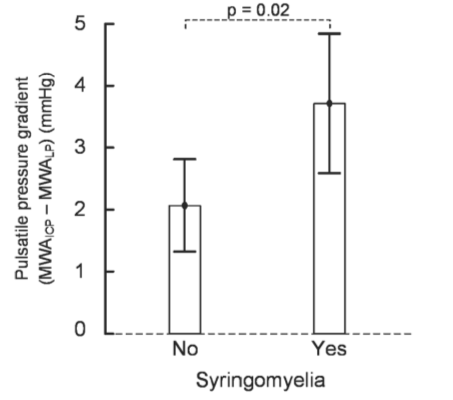
\includegraphics[width=0.4\linewidth]{figures/Eide_pressure_Syrinx}
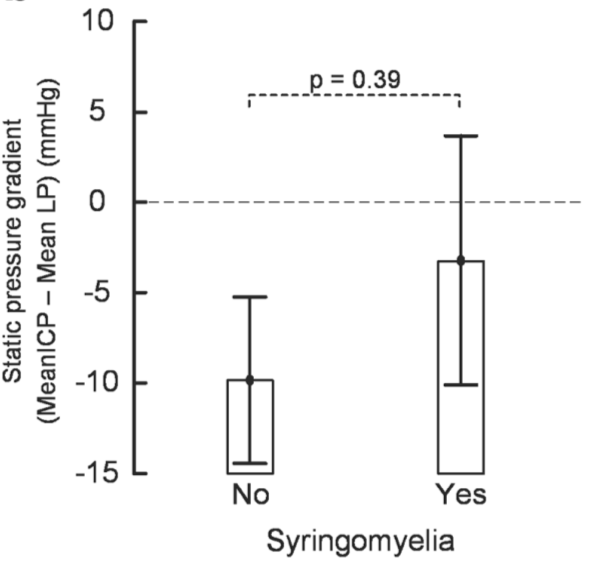
\includegraphics[width=0.375\linewidth]{figures/Eide_static}
\caption{Pulsatile (left) and static pressure gradient in patients as used in the study by Fri{\v{c}} and Eide \cite{Fric15}}\label{fig:Syrinx}
\end{figure}
\end{center}
The pulsatile intracranial pressure (ICP) as well as pulsatile pressure gradients were clearly abnormal or with boarderline values in 69 and 71 \% of Chiari I patients, respectively. Without any further speculation, it is interesting to note that these numbers are very close to the number of Chiari I patients that develops a syrinx. The median pressure difference in patients with abnormal pressure gradient were $2.6$ mm Hg between the intracranial CSF pressure and the lumbar (LP) CSF pressure. The actual mean static ICP was measured to a median of $7.1$ mmHg for the patients (range -0.7 -- 13.0), whereas the median of the mean lumbar pressure LP in the patients were $15.1$ mm Hg. Czosnyka and Pickard \cite{Czos04} reported ICP for healthy adult subjects to be $7-15$ mm Hg. Williams \cite{Will76} measured pressure up to $70$ mm Hg and $97$ mmHg in the SAS in the cisternal (just below the cerebellum) and lumbar region, respectively during coughing. Sansur et al. \cite{Sans03} measured the SAS pressure at the L5-level and found pressures up to $125$ mm Hg in patients coughing. The baseline pressures for healthy subjects were reported to be 8.6 -- 13.4 mm Hg.  
\\
\\
\begin{center}
\begin{figure}[!ht]
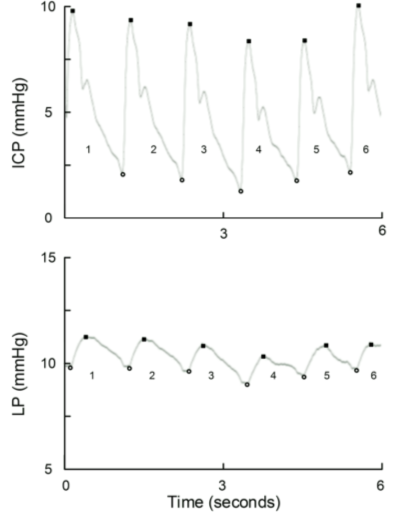
\includegraphics[scale=0.5]{figures/ICP_and_LP}
\caption{Intracranial (ICP) and lumbar (LP) pressure measured simultaneuously by Fri{\v{c}} and Eide}\label{fig:ICP_and_LP}
\end{figure}
\end{center}

\subsection{Applicability of medical measurements} \label{sec:AppMed}
From the modeling point of view, pressure measurements are of high interest in prescribing the correct boundary conditions at the top and bottom of the cord and SAS model. There are some challenges however. From our understanding, the main focus in most of these studies seem to be to measure pressure differences in Chiari patients \textit{compared} to healthy subjects. As showed by all studies in the previous section, altered pressure environment, and thus altered CSF dynamics is somehow related to syringomyelia. However, from a CFD point of view, the actual values of the pressure is also of high interest, and in particular the pressure difference between the Intracranial region and the lumbar region for a specific patient. Simultaneous measurements of ICP and LP was measured for the first time by Fri{\v{c}} and Eide \cite{Fric15}. They measured the pressure over night in subjects laying down. The mean LP was found to have a median value 8mmHg higher than the mean ICP. In addition to this, the pressure was always higher at the Lumbar region as depicted in figure \ref{fig:ICP_and_LP}. From the fluid mechanics point of view, this implies flow in the cranial direction at all times since no hydrostatic pressure should be present when laying down. This is in contradiction to results obtained by Haughton/Bruker (not published? (Brucker ASSR 2015.pptx)) where the net flux seem to be in the caudal direction. As for now, these measurements can probably be used for prescribing a normalized pressure waveform at the inlet, but to the authors opinion the actual pressure measurements can not to be used as boundary conditions to obtain reliable results. 
\\
\\
(Comment on experiments by Martin et al. \cite{Mart09Syrinx})?


\section{CSF velocities in syringomyelia}
Substantial flow within the syrinx have been reported, e.g. by Brugi{\`e}res et al. (2000) \cite{Brug00} where large syrinxes (graded A or AB) had mean peak velocities of 2.93 cm/s, and small syrinxes (graded B or C) had mean peak velocities of 1.5 cm/s. Haughton/Brucker reported flow up to 3.1 cm/s inside the syrinx in an assessment of CSF velocities and Cord Motion Before and After Chiari 1 Decompression. (Raw data available xxx). Fluid flow within the syrinx is also supported by Pinna et al. (2000) \cite{Pinn00}, and it was also pointed out that flow direction inside the syrinx did not neccessarily parallel with those observed in the SAS, and that these patterns may vary from patient to patient. 
\\
\\
We hypothesized that FSI-effects (deformation and pressure wave propagation) was at least partially responsible for the syrinx velocities reported in the literature.

xxx ALSO READ 5, 13, 21, 45 from Karen xxx
\begin{center}
\begin{figure}[!ht]
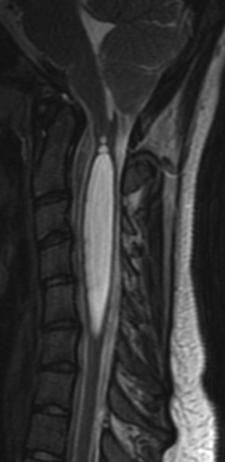
\includegraphics[width=0.51\linewidth]{figures/Syrinx_Subject} 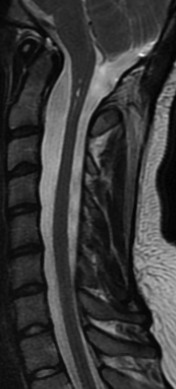
\includegraphics[width=0.474\linewidth]{figures/Syrinx_PostOp}
\centering{\caption{MRI image of 14 year old female subject before and 10 months after decompression. Note the withdrawal of the cerebellar tonsils in the post-operative image on the right}}
\end{figure}
\end{center}
In Brucker/Haughton CSF flow was measured with PCMR on three different stages: Pre-operative, 2 months post-operative and 10 months post-operative when the patient had no remaining symptoms. The peak velocity was reported to be 9.4 cm/s in the caudal direction for the pre-operative case. The velocities varied a lot over a cross-section of the cord, meaning the peak velocity 9.4 cm/s is not representative for the general velocity in the SAS. For the Cross section depicted in figure \ref{fig:CrossS}
the maximal velocities were registered at the upper left and upper right part of the circle. Along the axis of the cord, velocities in these areas lies around 4-6 cm/s. 
\begin{figure}[!h]
\begin{center}
\includegraphics[scale=4]{figures/brucker}
\caption{Cross-section of the spinal cord. The bottom of this cross-section is towards the face and the top is towards to the neck}\label{fig:CrossS}
\end{center}
\end{figure}
\begin{figure}[!h]
\begin{subfigure}[b]{0.5\linewidth}
\begin{center}
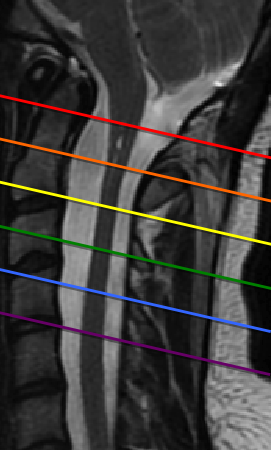
\includegraphics[width=0.7\linewidth]{figures/Syrinx_Levels}
\caption{Levels (from top to bottom) C1-C2, C2, C2-C3, C3, C3-C4 and C4-C5 of the spinal cord}
\end{center}
\end{subfigure}
\begin{subfigure}[b]{0.5\linewidth}
\begin{center}
\includegraphics[width=0.75\linewidth]{figures/mesh_coarse}
\caption{Coarse version of the computational mesh}
\end{center}
\end{subfigure}
\end{figure}
\begin{figure}[!h]
\begin{subfigure}[b]{0.5\linewidth}
\begin{center}
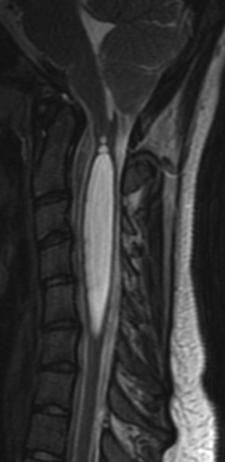
\includegraphics[width=0.7\linewidth]{figures/Syrinx_Subject}
\caption{Cord with fluid filled syrinx}
\end{center}
\end{subfigure}
\begin{subfigure}[b]{0.5\linewidth}
\begin{center}
\includegraphics[width=0.75\linewidth]{figures/mesh_3mm_coarse}
\caption{Computational mesh with a fluid filled cavity}
\end{center}
\end{subfigure}
\caption{Comparison of the spinal cord an the coarsest versions of the computaitonal meshes}
\end{figure}

\clearpage
\section{A note on interface conditions}
Since we want continuity of stresses on the interface, we use the divergence form \eqref{Momentum} of the momentum equation, to obtain these when integrating by parts. For the outflow and inflow boundaries for the fluid the pseudo traction condition are the condition of interest. The unknown shear term $\mathbf{n} \cdot (\nabla \mathbf{v}^T)$ should then be added to the bilinear form in the variational formulation. I.e with the pseudo traction condition we have
\begin{alignat}
\sigma \cdot \mathbf{n} = -p \mathbf{n} + \mu ( \nabla \mathbf{v} + (\nabla \mathbf{v})^T )\cdot \mathbf{n} & = \big{[}-p\mathbf{n} && + \mu \mathbf{n} \cdot \nabla \mathbf{v} \big{]} &&& +\mathbf{n} \cdot (\nabla \mathbf{v} ^T) \\
& = \big{[} -p\mathbf{n} && + \mu \pdi{\mathbf{v}}{n}\big{]} &&& +\mathbf{n} \cdot (\nabla \mathbf{v} ^T) \\
& = && -p_0 \mathbf{n}\ &&& +\mathbf{n} \cdot (\nabla \mathbf{v}^T) \label{BoundaryTerm}
\end{alignat}
It should be noted that the \textit{grad} function in FEniCS is in fact given such that grad(v) $= (\nabla \mathbf{v} )^T$, and the extra term in \eqref{BoundaryTerm} can be written 
\begin{cverbatim}
grad(v).T*n
\end{cverbatim}
in FEniCS. So far we have only dealt with symmetric operations regarding this function and therefore this distinction did not have to be made before this point. 
\\
Similarly, the term
\begin{align}
\pdi{\mathbf{U}}{n}
\end{align}
can in fact be included in the variational form by adding the term
\begin{cverbatim}
k*inner(grad(w('-'))*n('-'),psi('-'))*dS(5)
\end{cverbatim}
to the domain bilinear form aDF in section \ref{sec:FEniCS}. And
\begin{cverbatim}
inner(grad(U('-'))*n('-'),psi('-'))*dS(5)
\end{cverbatim}
 to the linear form LDF in the same set of equations. The interface have been given the value 5 and ('-') is used to distinguish variables in the fluid domain from the solid domain.This should give no restriction on $\mathbf{U}$ except that it will be continuous over the interface. These terms were omited in the valitation of the solver. The inclusion of these terms gave a small effect on displacements without a syrinx, but close to no effect on syrinx velocity or displacements in the presence of a syrinx. Deviations in x-displacements from the benchmark-case could arise by the fact that these terms were left out in that section, but this is something that will not be further investigated at the present time, and we keep these terms in the following simulations.
\\
\\
\section{Results, elastic cord}


The previously described models based on a elastic and poroelastic cord is used on a geometry describing idealized versions of the spinal cord. The meshes have the same dimensions as found in previous work by Dr{\o}sdal (2011), \cite{Dros11}. The height of the model is 60mm, and the spinal cord have a radius of 5mm. The distance from the cord to the dura mater is 4 mm, and this space is where CSF flows. The fluid cavity, where free fluid flow is allowed, is placed in the centre of the model, extending between heigths 10mm and 50mm in the longitudinal direction. We investigate three cases: No syrinx, a case with syrinx 1 mm radius and a syrinx with 3 mm radius.  
\\
\\
First, a sinusodial varying pressure was applied to the boundaries with a maximum of 20 Pa difference between top and bottom. This applied pressure gradient was reported by Dr{\o}sdal to result in peak velocities of around 5-6 cm/s assuming a rigid, but porous cord. The Simulations were run 10 cycles where a steady state was reached. Quantities of interest are the peak velocity in the SAS, max$|\mathbf{v}|$, the peak velocity inside the syrinx in the spinal canal, max$|\mathbf{v}_{sc}|$ and the maximum displacemen,t max$|\mathbf{U}|$ in both x- and y-direction.
\\
\\
\subsection{No syrinx}
\begin{table}[!h]
\begin{center}
  \begin{tabular}{l | l | l | l | l | l }
    $N_x$ & $N_y$ & dofs & max$|\mathbf{v}|$[cm/s] & max$|\mathbf{U}_x|$[mm] & max$|\mathbf{U}_y|$[mm] \\ \hline
    18  & 30 & 6281 & 5.68 & 0.003 & 0.02 \\ \hline
	36  & 60 & 24437 & 5.63 & 0.003 & 0.02 \\ \hline
	54  & 90  & 54473 & 5.63 & 0.003 & 0.02 \\ \hline
    \hline
  \end{tabular}
  \end{center}
  \caption{$E = 5 kPa, \Delta t = 0.002s, T = 10, \rho_s = 1.75\rho_f$}
\end{table}

\begin{table}[!h]
\begin{center}
  \begin{tabular}{l | l |  l | l | l | l }
    $N_x$ & $N_y$ & dofs & max$|\mathbf{v}|$[cm/s] & max$|\mathbf{U}_x|$[mm] & max$|\mathbf{U}_y|$[mm] \\ \hline
    18  & 30 & 6281 & 5.68 & 0.001 & 0.006 \\ \hline
	36  & 60 & 24437 & 5.62 & 0.001 & 0.006 \\ \hline
	54  & 90  & 54473 & 5.62 & 0.001 & 0.006 \\ \hline
    \hline
  \end{tabular}
  \end{center}
  \caption{$E = 16 kPa, \Delta t = 0.002s, T = 10, \rho_s = 1.75\rho_f$}
\end{table}
\begin{table}[!h]
\begin{center}
  \begin{tabular}{ l | l | l | l | l | l }
    $N_x$ & $N_y$ & dofs & max$|\mathbf{v}|$[cm/s] & max$|\mathbf{U}_x|$[mm] & max$|\mathbf{U}_y|$[mm] \\ \hline
    18  & 30 & 6281 & 5.67 & 3e-4 & 0.002 \\ \hline
	36  & 60 & 24437 & 5.61 & 3e-4 & 0.002 \\ \hline
	54  & 90 & 54473 & 5.62  & 3e-4 & 0.002  \\
    \hline
  \end{tabular}
  \end{center}
  \caption{$E = 62.5 kPa, \Delta t = 0.002s, T = 10, \rho_s = 1.75\rho_f$}
\end{table}
note: max displacement in x occurs at approx y=55 without syrinx. (y=40 w syrinx)
\clearpage
\subsection{1mm Syrinx}
\begin{table}[!h]
\begin{center}
  \begin{tabular}{l | l | l | l | l | l | l }
    $N_x$ & $N_y$ & dofs & max$|\mathbf{v}|$[cm/s] & max$|\mathbf{v}_{sc}|$[cm/s] & max$|\mathbf{U}_x|$[mm] & max$|\mathbf{U}_y|$[mm] \\ \hline
    18  & 30 & 6281 & 5.94 & 2.10 & 0.20 & 0.08 \\ \hline
	36 & 60 & 24437 & 5.91 & 2.14 & 0.20 & 0.08 \\ \hline
	54 & 90 & 54473 & 5.91 & 2.17 & 0.20 &  0.08 \\ \hline
	72 & 120& 96389 & 5.92 & 2.18 & 0.20 & 0.08 \\ \hline
    \hline
  \end{tabular}
  \end{center}
  \caption{$E = 5 kPa, \Delta t = 0.002s, T = 10s, \rho_s = 1.75 \rho_f$}
\end{table}

\begin{table}[!h]
\begin{center}
  \begin{tabular}{l | l | l | l | l | l | l }
    $N_x$ & $N_y$ & dofs & max$|\mathbf{v}|$[cm/s] & max$|\mathbf{v}_{sc}|$[cm/s] & max$|\mathbf{U}_x|$[mm] & max$|\mathbf{U}_y|$[mm] \\ \hline
    18  & 30 & 6281 & 5.76 & 0.57 & 0.05 & 0.02 \\ \hline
	36 & 60 & 24437 & 5.68 & 0.57 & 0.05 & 0.02 \\ \hline
	54 & 90 & 54473 & 5.69 & 0.58 & 0.05 & 0.02 \\ \hline
	72 & 120 & 96389& 5.70 & 0.58 & 0.05 & 0.02 \\ \hline
    \hline
  \end{tabular}
  \end{center}
  \caption{$E = 16 kPa, \Delta t = 0.002s, T = 10s, \rho_s = 1.75 \rho_f$}
\end{table}


\begin{table}[!h]
\begin{center}
  \begin{tabular}{l | l | l | l | l | l | l }
    $N_x$ & $N_y$ & dofs & max$|\mathbf{v}|$[cm/s] & max$|\mathbf{v}_{sc}|$[cm/s] & max$|\mathbf{U}_x|$[mm] & max$|\mathbf{U}_y|$[mm] \\ \hline
    18  & 30 & 6281 & 5.69 & 0.14 & 0.01 & 0.005 \\ \hline
	36 & 60 & 24437 & 5.63 & 0.14 & 0.01 & 0.005 \\ \hline
	54 & 90 & 54473 & 5.64 & 0.14 & 0.01 &  0.005 \\ \hline
	72 & 120 & 96389& 5.64 & 0.14 & 0.01 & 0.005 \\ \hline
    \hline
  \end{tabular}
  \end{center}
  \caption{$E = 62.5 kPa, \Delta t = 0.002s, T = 10s, \rho_s = 1.75 \rho_f$}
\end{table}
Discuss results
\subsection{3mm Syrinx}
\begin{table}[!h]
\begin{center}
  \begin{tabular}{l | l | l | l | l | l | l }
    $N_x$ & $N_y$ & dofs & max$|\mathbf{v}|$[cm/s] & max$|\mathbf{v}_{sc}|$[cm/s] & max$|\mathbf{U}_x|$[mm] & max$|\mathbf{U}_y|$[mm] \\ \hline
    18  & 30 & 6281 & 7.62 & 2.34 & 1.30 & 0.24 \\ \hline
	36 & 60 & 24437 & 7.15 & 2.54 & 1.13 & 0.23 \\ \hline
	54 & 90 & 54473 & 7.05 & 2.61 & 1.10 &  0.22 \\ \hline
	72 & 120& 96389 & 7.01 & 2.78 & 1.07 & 0.22 \\ \hline
    \hline
  \end{tabular}
  \end{center}
  \caption{$E = 5 kPa, \Delta t = 0.002s, T = 10s, \rho_s = 1.75 \rho_f$}
\end{table}

\begin{table}[!h]
\begin{center}
  \begin{tabular}{l | l | l | l | l | l | l }
    $N_x$ & $N_y$ & dofs & max$|\mathbf{v}|$[cm/s] & max$|\mathbf{v}_{sc}|$[cm/s] & max$|\mathbf{U}_x|$[mm] & max$|\mathbf{U}_y|$[mm] \\ \hline
    18  & 30 & 6281 & 6.11 & 0.79 & 0.34 & 0.06 \\ \hline
	36 & 60 & 24437 & 6.01 & 0.83 & 0.33 & 0.06 \\ \hline
	54 & 90 & 54473 & 6.00 & 0.84 & 0.33 & 0.06 \\ \hline
	72 & 120& 96389 & 6.00 & 0.85 & 0.33 & 0.06 \\ \hline
    \hline
  \end{tabular}
  \end{center}
  \caption{$E = 16 kPa, \Delta t = 0.002s, T = 10s, \rho_s = 1.75 \rho_f$}
\end{table}
\begin{table}[!h]
\begin{center}
  \begin{tabular}{l | l | l | l | l | l | l }
    $N_x$ & $N_y$ & dofs & max$|\mathbf{v}|$[cm/s] & max$|\mathbf{v}_{sc}|$[cm/s] & max$|\mathbf{U}_x|$[mm] & max$|\mathbf{U}_y|$[mm] \\ \hline
    18  & 30 & 6281 & 5.79 & 0.21 & 0.07 & 0.01 \\ \hline
	36 & 60 & 24437 & 5.70 & 0.21 & 0.07 & 0.01 \\ \hline
	54 & 90 & 54473 & 5.71 & 0.21 & 0.07 & 0.01 \\ \hline
	72 & 120& 96389 &  &  &  &  \\ \hline
    \hline
  \end{tabular}
  \end{center}
  \caption{$E = 62.5 kPa, \Delta t = 0.002s, T = 10s, \rho_s = 1.75 \rho_f$}
\end{table}

\begin{center}
\begin{figure}[!h]
\includegraphics[width=0.5\linewidth]{figures/E5000/Cord_1mm_ref3_E500_pressure}
\includegraphics[width=0.5\linewidth]{figures/E5000/Cord_ref3_E500_pressure}
\caption{Pressure fields at t=9.35 with E = 5kPa for a thin (radius 1mm) and thick (radius 3mm) syrinx. The pressure vector in the elastic cord have been set to 0. The pressure field inside the syrinx arises due to cord discplacements. The pressure gradient is in the opposite direction inside the syrinx causing flow in the opposite direction as compared to the outside SAS.}\label{fig:Cord_pressure}
\end{figure}
\end{center}
\clearpage
\section{Results, poroelastic cord}
\begin{table}[!h]
\begin{center}
  \begin{tabular}{ l | l | l | l | l }
    max$|\mathbf{v}|$[cm/s] & max$|\mathbf{U}_x|$[mm] & max$|\mathbf{U}_y|$[mm] & max$|\mathbf{q}|$[cm/s] & max$|\mathbf{q}|_0$[cm/s]\\ \hline
    5.67 & 2e-4 & 0.002 & 1.06e-7 & 3.4e-9 \\ \hline
    \hline
  \end{tabular}
  \end{center}
  \caption{$E = 62.5 kPa, \Delta t = 0.002s, T = 10, \rho_s = 1.75\rho_f$, $[N_x,N_y]=[18,30]$}
\end{table}
\begin{table}[!h]
\begin{center}
  \begin{tabular}{ l | l | l | l | l }
    max$|\mathbf{v}|$[cm/s] & max$|\mathbf{U}_x|$[mm] & max$|\mathbf{U}_y|$[mm] & max$|\mathbf{q}|$[cm/s] & max$|\mathbf{q}|_0$[cm/s]\\ \hline
    5.62 & 2e-4 & 0.002 & 2.42e-7 & 3.4e-9 \\ \hline
    \hline
  \end{tabular}
  \end{center}
  \caption{$E = 62.5 kPa, \Delta t = 0.002s, T = 10, \rho_s = 1.75\rho_f$, $[N_x,N_y]=[54,90]$}
\end{table}

\section{The effect of asymmetric pressure}
As mentioned in section \ref{sec:AppMed}, pressure measurements comparing the top and bottom of the cord is hard to obtain. If the temporal data in figure \ref{fig:ICP_and_LP} can be trusted the temporal variation in the lumbar region is almost negligible compared to the wave amplitude in the cranial region. For this reason, we use the ICP measurements as pressure difference between the top and bottom of the model and scale this data to obtain approximately expected CSF velocities. However, it should be noted that pressure measurements were done in the lumbar region, lower than the bottom part of the computational model presented here, and therefore the wave amplitude would not have been damped as much as down at the lumber region. This is by no means perfect, but in light of theories describing formations of a syrinx, it models a more realistic case than prescribing symmetric pressure.
\\
\\
The applied pressure was obtained by extracting raw data from ICP measurements over one representative cycle (1.16 s) and fitting to a 5-th degree spline. The spline does not capture all oscillations but is reasonable within the limitations described above. The pressure were set to 0 on the bottom of the cord. Both boundary conditions were set with the Pseudo-traction condition previously described. 
\begin{figure}[!h]
\begin{center}
\includegraphics[width=\linewidth]{figures/Boundary_conditions}
\caption{Pressure difference between top and bottom of the cord in comparison to measured ICP by Eide. In order to compare pressure charateristics, the sine function have been stretched out to match the period T=1.16 from the measured data. xxx DECIDE magnitude of Spline xxx}
\end{center}
\end{figure}
\section{Discussion}
Our experiments have given further evidence that FSI-effects on CSF-dynamics are negligible models of healthy subjects. A 10-fold increase in Youngs modulus gave only a decrease in 0.01 cm/s for these models, and no visible effect on CSF-dynamics. Cord displacements vary approximately linear with Youngs modulus which would be expected with a linear elasticity model, and the greatest displacements were only 3$\mu$m and 20$\mu$m in the radial and axial directions, respectively.
\\
\\
The presence of a syrinx, leaves only a small segment of spinal cord tissue between it and the surrounding SAS. This allows for greater displacements of the cord and thus fluid movement inside the syrinx. 
\section{Limitations}
Kent Evju, turbulence. \\
Martin2002, Eide pressure, CSF production, sinusoidal \\
Discuss Eide in light of Bertram reflections. \\
Effect of Pia mater
